\section{DMR Einführung \& Ursprung} \label{sec:ursprung}
DMR kurz für \emph{digital mobile radio} ist ein digitaler Funkstandard für Sprech- und Datenfunk. Das heißt, die Sprache wird nicht direkt über FM o.a. auf einem Kanal übertragen, sondern erst digitalisiert und mit einem Verlustbehafteten Codec codiert und dann als Datenpaket übertragen. Dies ermöglicht es bei jedem Ruf zusätzliche Informationen wie Quelle und Ziel des Rufs mitzuübertragen.

DMR wurde als Ersatz für den analogen Bündelfunk in der kommerziellen Anwendung entwickelt. Ein klassisches Beispiel für den kommerziellen Einsatz von DMR wäre ein Verkehrsflughafen. Damit ist nicht der Flugfunk auf dem Feld und in der Luft gemeint, sondern der Funkbetrieb zwischen dem ganzen Bodenpersonal. 

Auf so einem Flughafen arbeiten sehr viele Leute mit sehr unterschiedlichen Aufgaben. Da hätten wir (ohne Anspruch auf Vollständigkeit)
\begin{itemize}
 \item Die Reinigungskolonne,
 \item die Sicherheitsleute wie Gepäckkontrolle oder Wachschutz,
 \item das Vorfeld, also die Betankung, die Gepäckverladung \& das Catering, 
 \item die Betriebsfeuerwehr und
 \item die Zentrale.
\end{itemize}

All diese Mitarbeiter bekommen ein Funkgerät und sollen die folgenden Möglichkeiten haben:
\begin{itemize}
 \item Direkte Kommunikation zur Zentrale, alle Personen sollen die Zentrale erreichen können.
 \item Direkte Kommunikation zwischen zwei Personen innerhalb ihrer Gruppe ohne das andere Gruppen gestört werden. D.h., die Reinigungskolonne sollte sich untereinander absprechen können ohne die Betriebsfeuerwehr zu stören.
 \item Sog. Gruppenrufe einer Person an eine ganze Gruppe. Zum Beispiel die Zentrale an die gesamte Betriebsfeuerwehr. Aber auch ein Anruf eines Wachschützers an alle anderen Wachschützer um zum Beispiel Hilfe anzufordern. 
 \item Die Alarmierung Aller, einer ganzen Gruppe oder einzelner Personen durch die Zentrale (wird im Amateurfunk nicht verwendet).
\end{itemize}
 
Gleichzeitig ist so ein Flughafen ein riesiges Gelände. D.h., nicht alle Mitarbeiter können alle anderen Mitarbeiter direkt erreichen. Es müssen also Repeater aufgestellt werden, damit das gesamte Gelände per Funk abgedeckt ist, vor allem die Innenräume. Daher wird häufig in jedem Gebäude mindestens ein Repeater aufgestellt. 

Vergleicht man nun die Ansprüche dies Kommunikationsnetzes mit dem klassischen FM-Repeaterbetrieb (Abs. \ref{sec:vorwissen}) wird schnell deutlich, dass es sehr schwierig wird dieses Konzept per analog FM-Repeater umzusetzen, vor allem wenn mehrere Repeater in einem Netz (ähnlich Echolink) verbunden sind. Jede Kommunikation zwischen zwei Personen würde dann aber das gesamte Kommunikationsnetz belegen. 

Besser wäre es, wenn nur jene Repeater aktiv würden, die für die Kommunikation zwischen zwei Teilnehmern nötig sind. Dann stünden alle anderen Repeater für weitere Verbindungen bereit. Dieses Routing von Verbindungen sollte aber automatisch geschehen, da die zwei Teilnehmer nicht immer wissen werden, wo sich die jeweils andere Person befindet und somit mit welchem Repeater sie sich verbinden müssen. 

Um solche komplexen Kommunikationsnetze realisieren zu können ohne, dass der Teilnehmer detailliertes Wissen über dessen physische Struktur\footnote{Wissen darüber wo sich welcher Repeater befindet und wo sich welche Teilnehemer aufhalten.} benötigen, wurde DMR entwickelt.

\begin{merke}
 DMR hat mehr Ähnlichkeit mit einem Telefonnetz mit zusätzlichen Gruppenruf (anstatt ausschließlich eins-zu-eins Verbindungen) als mit klassischem FM-Repeaterbetrieb.
\end{merke} 

Das heißt, jeder Teilnehmer und damit dessen Funkgerät besitzt eine eindeutige Nummer\index{DMR-ID}. Diese Nummer liegt im Bereich $1$--$16777215$. Und wie bei einem gewöhnlichen Telefonnetz, kann ein Teilnehmer einen Anderen mit seiner Nummer direkt anrufen. Dies wird \adef{Direktruf} oder auch \adef{Private Call} genannt.

Außerdem werden Gruppen definiert, die auch wieder ihre eigene Nummer erhalten. Die sog. \adef{Sprechgruppe} oder auch \adef{Talk Group} (\emph{TG}). Diese Sprechgruppen dienen dazu alle Mitarbeiter einer bestimmten Gruppe (z.B., den Wachschutz, die Betriebsfeuerwehr, etc.) gleichzeitig erreichen zu können. Das heißt, das Funkgerät einer Reinigungskraft muss wissen, dass es auf die Gruppenrufe der Sprachgruppe \emph{Reinigung} reagieren muss aber alle anderen Sprechgruppen ignorieren soll. 

\begin{merke}
 Dieser Punkt ist sehr wichtig: Das DMR Netz selbst weiß nicht, welcher Teilnehmer zu welcher Gruppe gehört oder nicht. Das Funkgerät des Teilnehmers wird so konfiguriert, dass es nur auf bestimmte Gruppenrufe reagiert.
\end{merke}

\begin{figure}[!ht]
 \centering
 \documentclass{standalone}
\usepackage{tikz}
\usetikzlibrary{shapes.geometric}
\newcommand{\repeater}[3]{%
 \node ({#1}) at ({#2}) {%
  \begin{tikzpicture}%
   \draw [black,thick] (-.25,0) -- (0,0.5) -- (0.25,0) -- (-0.25,0);%
   \draw [black,thick,domain=-45:225] plot ({0.2*cos(\x)}, {0.5+0.2*sin(\x)});%
   \draw [black,thick,domain=-45:225] plot ({0.4*cos(\x)}, {0.5+0.4*sin(\x)});%
   \node (xxx) at (0,-.2) {{#3}};%
  \end{tikzpicture}%
 } %
}

\newcommand{\activerepeater}[3]{%
 \node ({#1}) at ({#2}) {%
  \begin{tikzpicture}%
   \draw [black,thick] (-.25,0) -- (0,0.5) -- (0.25,0) -- (-0.25,0);%
   \draw [red,thick,domain=-45:225] plot ({0.2*cos(\x)}, {0.5+0.2*sin(\x)});%
   \draw [red,thick,domain=-45:225] plot ({0.4*cos(\x)}, {0.5+0.4*sin(\x)});%
   \node (xxx) at (0,-.2) {{#3}};%
  \end{tikzpicture}%
 } %
}


\newcommand{\user}[3]{%
 \node ({#1}) at ({#2}) {%
  \begin{tikzpicture}%
   \draw [black,fill=black] (-.25,0) -- (0,0.5) -- (0.25,0) -- (-0.25,0);%
   \draw [black,fill=black] (0,.5) circle (.2); %
   \node (xxx) [text width=0.6cm, align=center] at (-.35cm,-.4) {{#3}};%
  \end{tikzpicture}%
 } %
}

\newcommand{\activeuser}[3]{%
 \node ({#1}) at ({#2}) {%
  \begin{tikzpicture}%
   \draw [red,fill=red] (-.25,0) -- (0,0.5) -- (0.25,0) -- (-0.25,0);%
   \draw [red,fill=red] (0,.5) circle (.2); %
   \node (xxx) [text width=0.6cm, align=center] at (-.35cm,-.4) {{#3}};%
  \end{tikzpicture}%
 } %
}

\begin{document}
 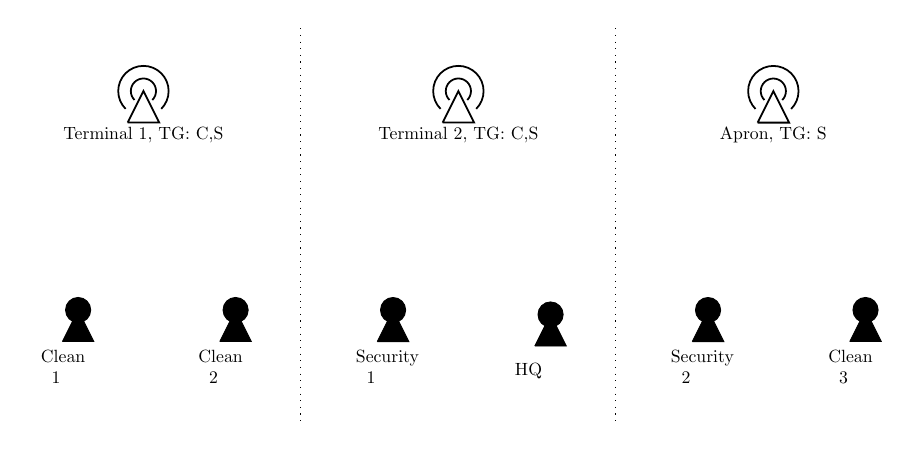
\begin{tikzpicture}[every node/.style={scale=.8}]
  \user{r1}{ 0,0}{Clean 1};
  \user{r2}{ 2,0}{Clean 2};	
  \draw[dotted] (3,4) -- (3,-1);
  \user{s1}{ 4,0}{Security 1};
  \user{z} { 6,0}{HQ};
  \draw[dotted] (7,4) -- (7,-1);
  \user{s2}{ 8,0}{Security 2};
  \user{r3}{10,0}{Clean 3};
  \repeater{R1}{1,3}{Terminal 1, TG: C,S};
  \repeater{R2}{5,3}{Terminal 2, TG: C,S};
  \repeater{R3}{9,3}{Apron, TG: S};
 \end{tikzpicture}
\end{document}

 \caption{Ein Beispielnetzwerk für den hypothetischen Flughafen. Es gibt drei Reinigungskräfte, zwei Sicherheitsleute und eine Zentrale. Um das gesammte Gelände abdecken zu können, werden drei Repeater benötigt einer in Terminal 1, einer in Terminal 2 und einer im Vorfeld.} \label{fig:exnet1}
\end{figure}

In Abbildung \ref{fig:exnet1} sei ein Beispielnetzwerk für den Flughafen dargestellt (in Wirklichkeit viel größer und komplexer). Nun stellen wir uns die Situation vor, dass die Reinigungskraft 1 \& 3 miteinander Sprechen wollen und gleichzeitig die Zentrale mit \emph{Sicherheit 1}. In einem einfachen analog Netz, bei dem alle Repeater einfach zusammengeschaltet wären, würde das Gespräch zwischen \emph{Reinigung 1} \& \emph{3} das gesamte Netz blockieren und die Verbindung zwischen \emph{Zentrale} und \emph{Sicherheit 1} wäre nicht möglich. 

\begin{figure}[!ht]
 \centering
 \documentclass{standalone}
\newcommand{\repeater}[3]{%
 \node ({#1}) at ({#2}) {%
  \begin{tikzpicture}%
   \draw [black,thick] (-.25,0) -- (0,0.5) -- (0.25,0) -- (-0.25,0);%
   \draw [black,thick,domain=-45:225] plot ({0.2*cos(\x)}, {0.5+0.2*sin(\x)});%
   \draw [black,thick,domain=-45:225] plot ({0.4*cos(\x)}, {0.5+0.4*sin(\x)});%
   \node (xxx) at (0,-.2) {{#3}};%
  \end{tikzpicture}%
 } %
}

\newcommand{\activerepeater}[3]{%
 \node ({#1}) at ({#2}) {%
  \begin{tikzpicture}%
   \draw [black,thick] (-.25,0) -- (0,0.5) -- (0.25,0) -- (-0.25,0);%
   \draw [red,thick,domain=-45:225] plot ({0.2*cos(\x)}, {0.5+0.2*sin(\x)});%
   \draw [red,thick,domain=-45:225] plot ({0.4*cos(\x)}, {0.5+0.4*sin(\x)});%
   \node (xxx) at (0,-.2) {{#3}};%
  \end{tikzpicture}%
 } %
}


\newcommand{\user}[3]{%
 \node ({#1}) at ({#2}) {%
  \begin{tikzpicture}%
   \draw [black,fill=black] (-.25,0) -- (0,0.5) -- (0.25,0) -- (-0.25,0);%
   \draw [black,fill=black] (0,.5) circle (.2); %
   \node (xxx) [text width=0.6cm, align=center] at (-.35cm,-.4) {{#3}};%
  \end{tikzpicture}%
 } %
}

\newcommand{\activeuser}[3]{%
 \node ({#1}) at ({#2}) {%
  \begin{tikzpicture}%
   \draw [red,fill=red] (-.25,0) -- (0,0.5) -- (0.25,0) -- (-0.25,0);%
   \draw [red,fill=red] (0,.5) circle (.2); %
   \node (xxx) [text width=0.6cm, align=center] at (-.35cm,-.4) {{#3}};%
  \end{tikzpicture}%
 } %
}

\begin{document}
 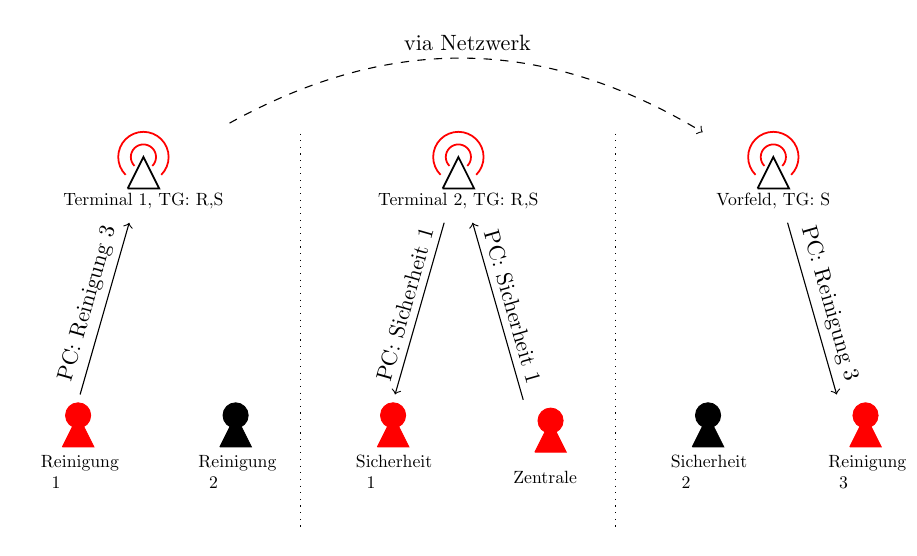
\begin{tikzpicture}[every node/.style={scale=.8}]
  \activeuser{r1}{ 0,0}{Reinigung 1};
  \user{r2}{ 2,0}{Reinigung 2};	
  \draw[dotted] (3,4) -- (3,-1);
  \activeuser{s1}{ 4,0}{Sicherheit 1};
  \activeuser{z} { 6,0}{Zentrale};
  \draw[dotted] (7,4) -- (7,-1);
  \user{s2}{ 8,0}{Sicherheit 2};
  \activeuser{r3}{10,0}{Reinigung 3};
  \activerepeater{R1}{1,3.5}{Terminal 1, TG: R,S};
  \activerepeater{R2}{5,3.5}{Terminal 2, TG: R,S};
  \activerepeater{R3}{9,3.5}{Vorfeld, TG: S};
  \draw[->] (r1) -- node[above,rotate=74] {PC: Reinigung 3} (R1);
  \path[->,dashed] (R1) edge [bend left] node[above] {via Netzwerk} (R3);
  \draw[->] (R3) -- node[above,rotate=-74] {PC: Reinigung 3} (r3);
  \draw[->] (z) -- node[above,rotate=-74] {PC: Sicherheit 1} (R2);
  \draw[->] (R2) -- node[above,rotate=74] {PC: Sicherheit 1} (s1);
 \end{tikzpicture}
\end{document}

 \caption{Zwei gleichzeitige Direktrufe (Private Calls, PC) in dem Beispielnetzwerk zwischen \emph{Reinigung 1 \& 3} sowie zwischen \emph{Zentrale} und \emph{Sicherheit 1}} \label{fig:exnet2}
\end{figure}

In einem DMR Netz hingegen, werden für einen Direktruf (Privat Call) nur jene Repeater verwendet, die dafür nötig sind. Dies ist in Abbildung \ref{fig:exnet2} zu sehen: \emph{Reinigung 1} startet einen Direktruf (Private Call) über ihren lokalen Repeater in \emph{Terminal 1}. Da das DMR Netzwerk weiß über welchen Repeater \emph{Reinigung 3} zuletzt aktiv war, wird der Direktruf vom DMR Netz über den Repeater auf dem Vorfeld etabliert. Der Repeater im Terminal 2 hingegen wird für diesen Direktruf nicht aktiv. Daher steht dieser Repeater weiterhin für weitere Kommunikation zur Verfügung. Dies nutzt die Zentrale um \emph{Sicherheit 1} per Direktruf zu erreichen. 

Solange das Gespräch zwischen \emph{Reinigung 1 \& 3} anhält sind aber die Repeater im Terminal 1 und auf dem Vorfeld belegt. D.h., die Zentrale kann \emph{Reinigung 2} und \emph{Sicherheit 2} nicht erreichen. 

Dies klingt schlimmer als es ist. Im Gegensatz zu klassischen Telefonaten gilt im DMR Netz ein Direktruf als unterbrochen sobald ein Teilnehmer die PTT Taste loslässt. Daher kann die Zentrale in den Umschaltpausen des Gespräches \emph{dazwischenrufen} und z.B. \emph{Sicherheit 2} erreichen. 

Im nächsten Beispiel (Abbildung \ref{fig:exnet3}) will die Zentrale alle Reinigungskräfte erreichen. Dazu macht sie einen Gruppenruf zur Sprechgruppe/Talk Group \emph{Reinigung} (R für Reinigung, S für Sicherheit). Damit erreicht sie die \emph{Reinigung 1 \& 2} problemlos, aber \emph{Reinigung 3} empfängt diesen Gruppenruf nicht. 

Dies liegt daran, dass das DMR Netz nicht weiß, welche Personen zu welcher Gruppe gehören. Da sich Reinigungskräfte üblicherweise nicht auf dem Vorfeld herumtreiben, hat der Repeater auf dem Vorfeld die Sprechgruppe \emph{Reinigung (R)} nicht \emph{abonniert} und leitet daher keine Gruppenrufe für diese Sprechgruppe weiter. 

\begin{figure}[p]
 \begin{subfigure}{\linewidth}
  \centering
  \documentclass{standalone}
\usepackage{tikz}
\usetikzlibrary{shapes.geometric}
\newcommand{\repeater}[3]{%
 \node ({#1}) at ({#2}) {%
  \begin{tikzpicture}%
   \draw [black,thick] (-.25,0) -- (0,0.5) -- (0.25,0) -- (-0.25,0);%
   \draw [black,thick,domain=-45:225] plot ({0.2*cos(\x)}, {0.5+0.2*sin(\x)});%
   \draw [black,thick,domain=-45:225] plot ({0.4*cos(\x)}, {0.5+0.4*sin(\x)});%
   \node (xxx) at (0,-.2) {{#3}};%
  \end{tikzpicture}%
 } %
}

\newcommand{\activerepeater}[3]{%
 \node ({#1}) at ({#2}) {%
  \begin{tikzpicture}%
   \draw [black,thick] (-.25,0) -- (0,0.5) -- (0.25,0) -- (-0.25,0);%
   \draw [red,thick,domain=-45:225] plot ({0.2*cos(\x)}, {0.5+0.2*sin(\x)});%
   \draw [red,thick,domain=-45:225] plot ({0.4*cos(\x)}, {0.5+0.4*sin(\x)});%
   \node (xxx) at (0,-.2) {{#3}};%
  \end{tikzpicture}%
 } %
}


\newcommand{\user}[3]{%
 \node ({#1}) at ({#2}) {%
  \begin{tikzpicture}%
   \draw [black,fill=black] (-.25,0) -- (0,0.5) -- (0.25,0) -- (-0.25,0);%
   \draw [black,fill=black] (0,.5) circle (.2); %
   \node (xxx) [text width=0.6cm, align=center] at (-.35cm,-.4) {{#3}};%
  \end{tikzpicture}%
 } %
}

\newcommand{\activeuser}[3]{%
 \node ({#1}) at ({#2}) {%
  \begin{tikzpicture}%
   \draw [red,fill=red] (-.25,0) -- (0,0.5) -- (0.25,0) -- (-0.25,0);%
   \draw [red,fill=red] (0,.5) circle (.2); %
   \node (xxx) [text width=0.6cm, align=center] at (-.35cm,-.4) {{#3}};%
  \end{tikzpicture}%
 } %
}

\begin{document}
  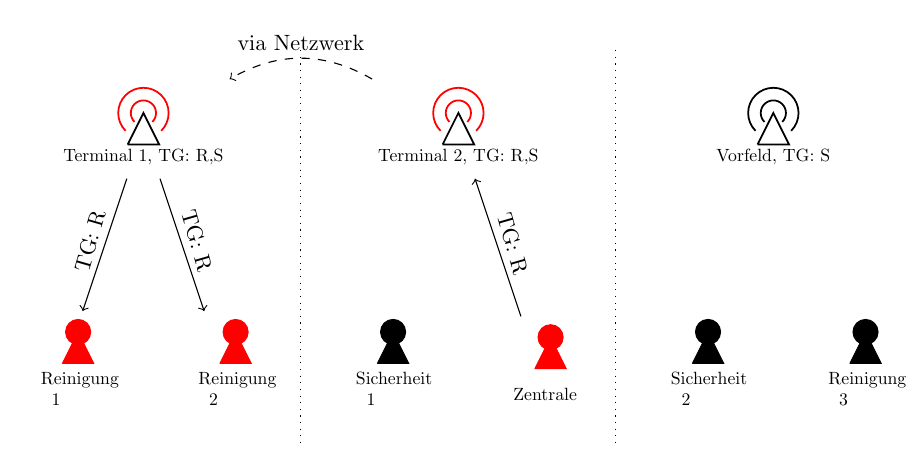
\begin{tikzpicture}[every node/.style={scale=.8}]
   \activeuser{r1}{ 0,0}{Reinigung 1};
   \activeuser{r2}{ 2,0}{Reinigung 2};	
   \draw[dotted] (3,4) -- (3,-1);
   \user{s1}{ 4,0}{Sicherheit 1};
   \activeuser{z} { 6,0}{Zentrale};
   \draw[dotted] (7,4) -- (7,-1);
   \user{s2}{ 8,0}{Sicherheit 2};
   \user{r3}{10,0}{Reinigung 3};
   \activerepeater{R1}{1,3}{Terminal 1, TG: R,S};
   \activerepeater{R2}{5,3}{Terminal 2, TG: R,S};
   \repeater{R3}{9,3}{Vorfeld, TG: S};
   \draw[->] (z) -- node[above,rotate=-74] {TG: R} (R2);
   \path[->,dashed] (R2) edge [bend right] node[above] {via Netzwerk} (R1);
   \draw[->] (R1) -- node[above,rotate=74] {TG: R} (r1);
   \draw[->] (R1) -- node[above,rotate=-74] {TG: R} (r2);
  \end{tikzpicture}
\end{document}

  \caption{Ein Gruppenruf zur Sprechgruppe \emph{Reinigung} von der Zentrale aus. Der Teilnehmer \emph{Reinigung 3} wird aber nicht erreicht, da der Vorfeldrepeater diese Sprechgruppe nicht abonniert hat.} \label{fig:exnet3}
 \end{subfigure}\vspace{0.5cm}
 \begin{subfigure}{\linewidth}
  \centering
  \documentclass{standalone}
\usepackage{tikz}
\usetikzlibrary{shapes.geometric}
\newcommand{\repeater}[3]{%
 \node ({#1}) at ({#2}) {%
  \begin{tikzpicture}%
   \draw [black,thick] (-.25,0) -- (0,0.5) -- (0.25,0) -- (-0.25,0);%
   \draw [black,thick,domain=-45:225] plot ({0.2*cos(\x)}, {0.5+0.2*sin(\x)});%
   \draw [black,thick,domain=-45:225] plot ({0.4*cos(\x)}, {0.5+0.4*sin(\x)});%
   \node (xxx) at (0,-.2) {{#3}};%
  \end{tikzpicture}%
 } %
}

\newcommand{\activerepeater}[3]{%
 \node ({#1}) at ({#2}) {%
  \begin{tikzpicture}%
   \draw [black,thick] (-.25,0) -- (0,0.5) -- (0.25,0) -- (-0.25,0);%
   \draw [red,thick,domain=-45:225] plot ({0.2*cos(\x)}, {0.5+0.2*sin(\x)});%
   \draw [red,thick,domain=-45:225] plot ({0.4*cos(\x)}, {0.5+0.4*sin(\x)});%
   \node (xxx) at (0,-.2) {{#3}};%
  \end{tikzpicture}%
 } %
}


\newcommand{\user}[3]{%
 \node ({#1}) at ({#2}) {%
  \begin{tikzpicture}%
   \draw [black,fill=black] (-.25,0) -- (0,0.5) -- (0.25,0) -- (-0.25,0);%
   \draw [black,fill=black] (0,.5) circle (.2); %
   \node (xxx) [text width=0.6cm, align=center] at (-.35cm,-.4) {{#3}};%
  \end{tikzpicture}%
 } %
}

\newcommand{\activeuser}[3]{%
 \node ({#1}) at ({#2}) {%
  \begin{tikzpicture}%
   \draw [red,fill=red] (-.25,0) -- (0,0.5) -- (0.25,0) -- (-0.25,0);%
   \draw [red,fill=red] (0,.5) circle (.2); %
   \node (xxx) [text width=0.6cm, align=center] at (-.35cm,-.4) {{#3}};%
  \end{tikzpicture}%
 } %
}

\begin{document}
  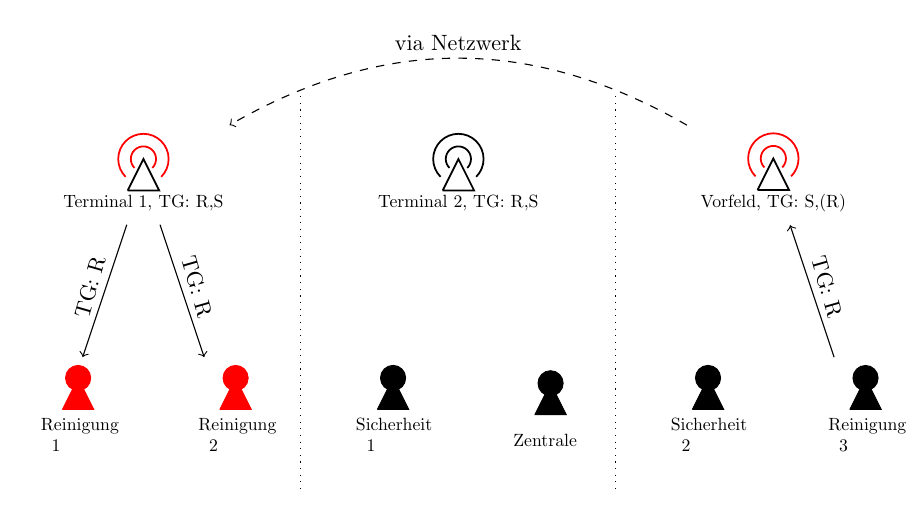
\begin{tikzpicture}[every node/.style={scale=.8}]
   \activeuser{r1}{ 0,0}{Reinigung 1};
   \activeuser{r2}{ 2,0}{Reinigung 2};	
   \draw[dotted] (3,4) -- (3,-1);
   \user{s1}{ 4,0}{Sicherheit 1};
   \user{z} { 6,0}{Zentrale};
   \draw[dotted] (7,4) -- (7,-1);
   \user{s2}{ 8,0}{Sicherheit 2};
   \user{r3}{10,0}{Reinigung 3};
   \activerepeater{R1}{1,3}{Terminal 1, TG: R,S};
   \repeater{R2}{5,3}{Terminal 2, TG: R,S};
   \activerepeater{R3}{9,3}{Vorfeld, TG: S,(R)};
   \draw[->] (r3) -- node[above,rotate=-74] {TG: R} (R3);
   \path[->,dashed] (R3) edge [bend right] node[above] {via Netzwerk} (R1);
   \draw[->] (R1) -- node[above,rotate=74] {TG: R} (r1);
   \draw[->] (R1) -- node[above,rotate=-74] {TG: R} (r2);
  \end{tikzpicture}
\end{document}

  \caption{Teilnehmer \emph{Reinigung 3} abonniert die Sprechgruppe \emph{Reinigung} temporär auf dem Vorfeldrepeater, indem er einen Gruppenruf zu dieser Sprechgruppe startet.} \label{fig:exnet4a} 
 \end{subfigure}\vspace{.5cm}
 \begin{subfigure}{\linewidth}
  \centering
  \documentclass{standalone}
\usepackage{tikz}
\usetikzlibrary{shapes.geometric}
\newcommand{\repeater}[3]{%
 \node ({#1}) at ({#2}) {%
  \begin{tikzpicture}%
   \draw [black,thick] (-.25,0) -- (0,0.5) -- (0.25,0) -- (-0.25,0);%
   \draw [black,thick,domain=-45:225] plot ({0.2*cos(\x)}, {0.5+0.2*sin(\x)});%
   \draw [black,thick,domain=-45:225] plot ({0.4*cos(\x)}, {0.5+0.4*sin(\x)});%
   \node (xxx) at (0,-.2) {{#3}};%
  \end{tikzpicture}%
 } %
}

\newcommand{\activerepeater}[3]{%
 \node ({#1}) at ({#2}) {%
  \begin{tikzpicture}%
   \draw [black,thick] (-.25,0) -- (0,0.5) -- (0.25,0) -- (-0.25,0);%
   \draw [red,thick,domain=-45:225] plot ({0.2*cos(\x)}, {0.5+0.2*sin(\x)});%
   \draw [red,thick,domain=-45:225] plot ({0.4*cos(\x)}, {0.5+0.4*sin(\x)});%
   \node (xxx) at (0,-.2) {{#3}};%
  \end{tikzpicture}%
 } %
}


\newcommand{\user}[3]{%
 \node ({#1}) at ({#2}) {%
  \begin{tikzpicture}%
   \draw [black,fill=black] (-.25,0) -- (0,0.5) -- (0.25,0) -- (-0.25,0);%
   \draw [black,fill=black] (0,.5) circle (.2); %
   \node (xxx) [text width=0.6cm, align=center] at (-.35cm,-.4) {{#3}};%
  \end{tikzpicture}%
 } %
}

\newcommand{\activeuser}[3]{%
 \node ({#1}) at ({#2}) {%
  \begin{tikzpicture}%
   \draw [red,fill=red] (-.25,0) -- (0,0.5) -- (0.25,0) -- (-0.25,0);%
   \draw [red,fill=red] (0,.5) circle (.2); %
   \node (xxx) [text width=0.6cm, align=center] at (-.35cm,-.4) {{#3}};%
  \end{tikzpicture}%
 } %
}

\begin{document}
  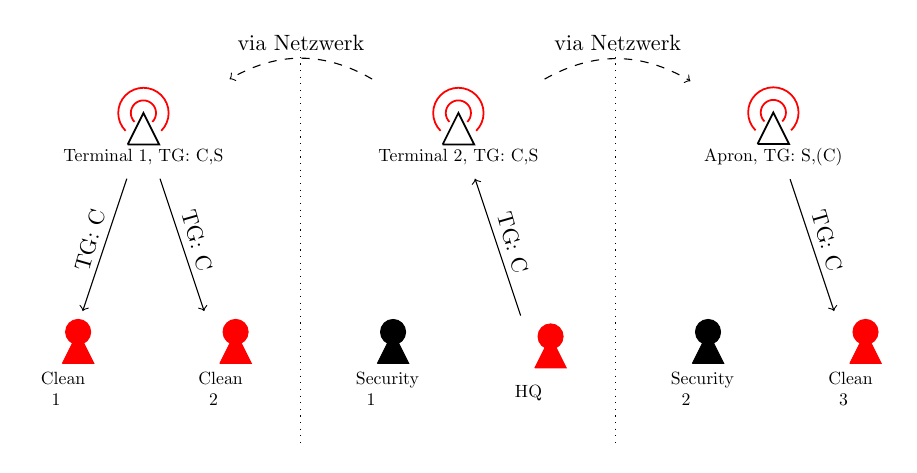
\begin{tikzpicture}[every node/.style={scale=.8}]
   \activeuser{r1}{ 0,0}{Clean 1};
   \activeuser{r2}{ 2,0}{Clean 2};	
   \draw[dotted] (3,4) -- (3,-1);
   \user{s1}{ 4,0}{Security 1};
   \activeuser{z} { 6,0}{HQ};
   \draw[dotted] (7,4) -- (7,-1);
   \user{s2}{ 8,0}{Security 2};
   \activeuser{r3}{10,0}{Clean 3};
   \activerepeater{R1}{1,3}{Terminal 1, TG: C,S};
   \activerepeater{R2}{5,3}{Terminal 2, TG: C,S};
   \activerepeater{R3}{9,3}{Apron, TG: S,(C)};
   \draw[->] (z) -- node[above,rotate=-74] {TG: C} (R2);
   \path[->,dashed] (R2) edge [bend right] node[above] {via Netzwerk} (R1);
   \path[->,dashed] (R2) edge [bend left] node[above] {via Netzwerk} (R3);
   \draw[->] (R1) -- node[above,rotate=74] {TG: C} (r1);
   \draw[->] (R1) -- node[above,rotate=-74] {TG: C} (r2);
   \draw[->] (R3) -- node[above,rotate=-74] {TG: C} (r3);
  \end{tikzpicture}
\end{document}

  \caption{Nach der temporären Abonnierung, ist nun der Teilnehmer \emph{Reinigung 3} auch auf dem Vorfeld erreichbar.} \label{fig:exnet4b}
 \end{subfigure}
 \caption{Temporäres Abonnement einer Sprechgruppe auf einem Repeater.} \label{fig:exnet4}
\end{figure}

Damit die Reinigungskraft 3 jedoch für Gruppenrufe erreichbar bleibt muss sie die Sprechgruppe \emph{Reinigung} auf dem Vorfeldrepeater temporär abonnieren. Dazu startet sie einen Gruppenruf zur Sprechgruppe \emph{Reinigung} vom Vorfeldrepeater aus (siehe Abb. \ref{fig:exnet4a}). Damit abonniert der Vorfeldrepeater diese Sprechgruppe für eine begrenzte Zeit\footnote{Diese Zeit wird auf jedem einzelnen Repeater konfiguriert. Üblich sind Zeiten zwischen $10$ und $30$ Minuten.} und wird während dieser Zeit Gruppenrufe dieser Sprechgruppe aussenden. 

Dieses temporäre Abonnement wird jedes mal erneuert oder wiederhergestellt, wenn ein Gruppenruf zu dieser Sprechgruppe von diesem Repeater initiiert wird. Das heißt, das Abonnement verlängert sich jedes mal, wenn \emph{Reinigung 3} einen Gruppenruf zur Sprechgruppe \emph{Reinigung} startet oder darauf antwortet\footnote{Das Antworten auf einen Gruppenruf ist technisch identisch zum Start eines neuen Gruppenrufs.}.

Mit diesen Beispielen sind die wichtigsten Grundbegriffe von DMR (DMR-ID, Talk Groups, Private sowie Group Call, Talk Group Abonnement) eingeführt und deren Verwendung in einem Beispiel DMR Netz erläutert worden. In den nächsten Absetzen wird die Verwendung von DMR im Amateurfunk beschrieben.

